\documentclass{article}
\usepackage{geometry}
 \geometry{
 a4paper,
 total={170mm,257mm},
 left=20mm,
 top=20mm,
 }

 \usepackage{mathptmx}
 \usepackage{amsmath}
 \usepackage{diagbox}
 \usepackage{booktabs}
\usepackage{colortbl}
\usepackage{amssymb}

\usepackage{hyperref}
\hypersetup{
    colorlinks=True,
    linkcolor={blue!20!black},
    filecolor=magenta,      
    urlcolor=cyan,
}


 \usepackage{caption}
\usepackage[export]{adjustbox} %% for picture frame
\usepackage[english]{babel}
\usepackage[utf8]{inputenc}
\usepackage{fancyhdr}


\pagestyle{fancy}
\fancyhf{}
\rhead{{Signal Analysis}}
\lhead{{Amrit Prasad Phuyal (PUL074BEX004)}}
\rfoot{\thepage}

%%% format and command for lab ans vhdl

%%% Formating And Command for Embedded Lab  VHDl
%% \ancode{caption}{Filename}


\usepackage{listings}
\usepackage{multicol}
\usepackage{mdframed}

\renewcommand{\lstlistlistingname}{List of MATLAB Codes}
\renewcommand{\lstlistingname}{MATLAB Code}

\setlength{\columnsep}{0.5cm}

\usepackage{xcolor}
\definecolor{codegreen}{rgb}{0,0.6,0}
\definecolor{codegray}{rgb}{0.3,0.3,0.3}
\definecolor{codepurple}{rgb}{0.58,0,0.82}
%\definecolor{backcolour}{rgb}{0.95,0.99,0.92}
\definecolor{backcolour}{rgb}{0,0,0}

\lstdefinestyle{MATLAB}{
  %backgroundcolor=\color{backcolour},  
  commentstyle=\color{codegreen},
  keywordstyle=\color{blue},
  numberstyle=\tiny\color{codegray},
  stringstyle=\color{codepurple},
  basicstyle=\ttfamily\small\color{black},
  breakatwhitespace=false,
  breaklines=true,
  captionpos=b,
  keepspaces=true,
  language=Matlab,
  numbers=left,
  numbersep=5pt,
  showspaces=false,
  frame = single,
  showstringspaces=false,
  showtabs=false,
  tabsize=3
}




\newcommand {\anscode}[2]{
  \lstinputlisting[style=MATLAB,nolol]{#2}

  \begingroup
  \captionof{lstlisting}{#1}
  \endgroup

}

%%% Formating And Command for Embedded Lab  VHDL
%%%%>>>>>>>........
%%%%%% include  Titles.%%%% use \input{./CP}%%%
%%%use """"""""    \CP{}{}{}{}   """" %%%% and 4 argument to craete Title page 
%%%%%%%%%%%%%%%%%%%%%%%%%%%%%%%%%%%%%%%%%%%%%%%%%%%%%%%%%%%%%%%%%
%%%argument number
%% 1=major header ## Course name 
%% 2=minor4 heading ## lab/assignmet no
%% 3=Title  ## Assignment or Lab title
%% 4=submitted to::## input receiver Name"
%%%%%%%%%%%%%%%%%%%%%%%%%%%%%%%%%%%%%%%%%%%%%%%%%%%%%%%%%%%%%%%%%


\usepackage{mathpazo} % Palatino font
\usepackage{graphicx}
\usepackage{float}

%%% format and command for lab ans c and assembly

\newcommand{\HRule}{\rule{\linewidth}{0.4mm}} % Defines a new command for horizontal lines, change thickness here



%----------------------------------------------------------------------------------------
%	TITLE PAGE
%----------------------------------------------------------------------------------------


\newcommand{\CP}[4]{ \begin{titlepage} % Suppresses displaying the page number on the title page and the subsequent page counts as page 1
		%%%%  univerdity logo%%
		\begin{figure}[H]
			\centering
			
\includegraphics[scale=0.13]{tulogo.jpg}
		\end{figure}
		%%% end university logo

		\center % Centre everything on the page

		%------------------------------------------------
		%	Headings
		%------------------------------------------------

		\textsc{\huge Institute of Engineering \\ Central Campus,Pulchowk}\\[1.5cm] % Main heading such as the name of your university/college

		\textsc{\Large #1}\\[0.5cm] % Major heading such as course name

		\textsc{\large #2}\\[0.5cm] % Minor heading such as assignment no./ lab no.

		%------------------------------------------------
		%	Title
		%------------------------------------------------

		\HRule\\[0.4cm]

		{\Huge\bfseries #3}\\[0.4cm] % Title of your document

		\HRule\\[1.5cm]

		%------------------------------------------------
		%	Author(s)
		%------------------------------------------------
		\vfill\vfill
		\begin{minipage}{0.4\textwidth}
			\begin{flushleft}
				\large{
				\textbf{Submitted BY:}\\
				{\normalsize AMRIT PRASAD PHUYAL}\\ % NAME
				{\normalsize Roll: PULL074BEX004}} % Roll
			\end{flushleft}
		\end{minipage}
		~
		\begin{minipage}{0.4\textwidth}
			\begin{flushright}
				\large
				\textbf{Submitted To:}\\
				{ \normalsize{#4}\\ }% recepent's  Name 
				{\normalsize Department of Electronics and Computer Engineering}
			\end{flushright}
		\end{minipage}

		%------------------------------------------------
		%	Date
		%------------------------------------------------

		\vfill\vfill\vfill % Position the date 3/4 down the remaining page

		{\large\today} % Date, change the \today to a set date if you want to be precise

		\vfill % Push the date up 1/4 of the remaining page

	\end{titlepage}
}
\DeclareUnicodeCharacter{2212}{-}

\begin{document}

%----------------------------------------------------------------------------------------
%	TITLE PAGE
%----------------------------------------------------------------------------------------
\CP{Signal Analysis}{All in One}
{Visualization of Signals, Fourier Series \& Transform, Convolution and Frequency Response}
{Department of Electronics and Computer Engineering}




%----------------------------------------------------------------------------------------
\pagenumbering{gobble}
\tableofcontents
\vspace{1in}
%\pagebreak
\listoffigures
\vspace{1in}
%\pagebreak
\lstlistoflistings
\pagebreak
\pagenumbering{arabic}


% \anscode{testing matolahb cod4e}{./CODES/sino.m}


% \begin{figure}[H]
%     \centering
%     \includegraphics[scale=1,cframe=blue 0.5pt 3pt]{./FIG/sino}
%     \caption{..sad gd }
% \end{figure}


%%%%%%%%%%%%%%%%%%%%%%%%%
%%%%%%%%%%%%%%%%%%%%%%%
\section{Signal Visualization}
Signal is a function of one or more independent variables, which contain some information.Analog signal is a continuous signal in which one time-varying quantity represents another time-based variable and denoted as $x(t), y(t)$.A digital signal is a signal that is used to represent data as a sequence of separate values at any point in time denoted as $ x[n], y[n]$.


\subsection{Sinusoidal Signal}
Sinusoidal signal is in the form of x(t) = A cos(${w}_{0}\,\pm \phi$) or A sin(${w}_{0}\,\pm \phi$).
In matlab \textbf{sin} and \textbf{cos} function are used to calculate sine and cosine values and \textbf{plot} function to plot continuous Sinusoidal signal. \textbf{hold on} \& \textbf{hold off} command is used to display both signal in single plot. Similarly \textbf{xlabel}, \textbf{ylabel} and \textbf{title} are used for Labeling purposes.

\anscode{Visualization of signal x(t) \& y(t)}{./CODES/sinu.m}
\begin{figure}[H]
    \centering
    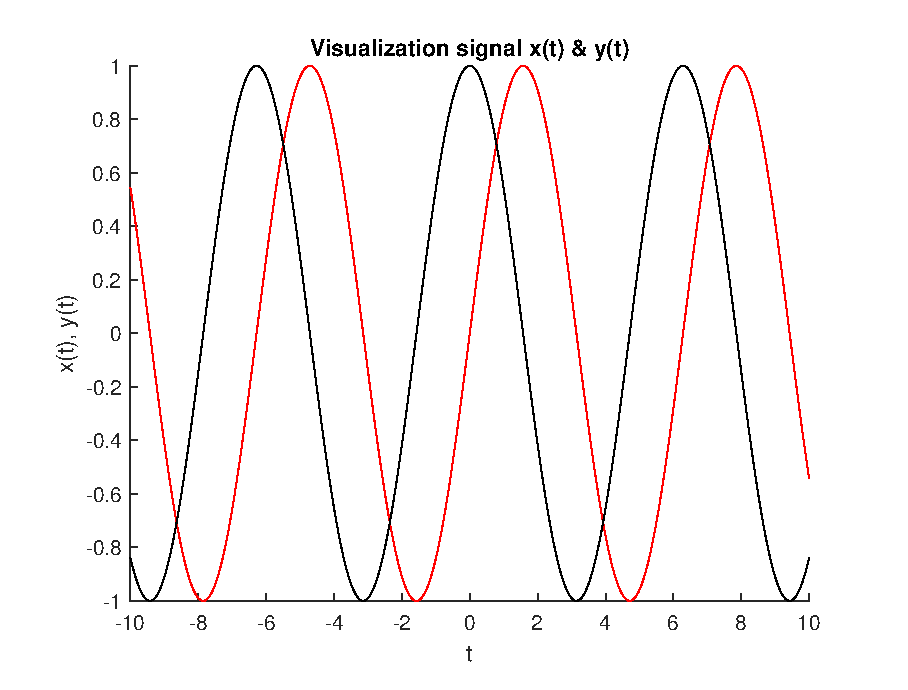
\includegraphics[scale=1.2,cframe=blue 0.5pt 3pt]{./FIG/sinu}
    \caption{Visualization of Sinusoidal signal }
\end{figure}


% %%%%%%%%%%%%%%%%%%%%%%%%%
% %%%%%%%%%%%%%%%%%%%%%%%

\subsection{Ramp Signal}
Ramp signal is denoted by $r[n]=an $and $r(t)=at$ for discrete and continuous signal. To plot discrete signal \textbf{stem} function is used in MATLAB.

\anscode{Discrete and Continuous ramp Signal}{./CODES/ramp.m}
\begin{figure}[H]
    \centering
    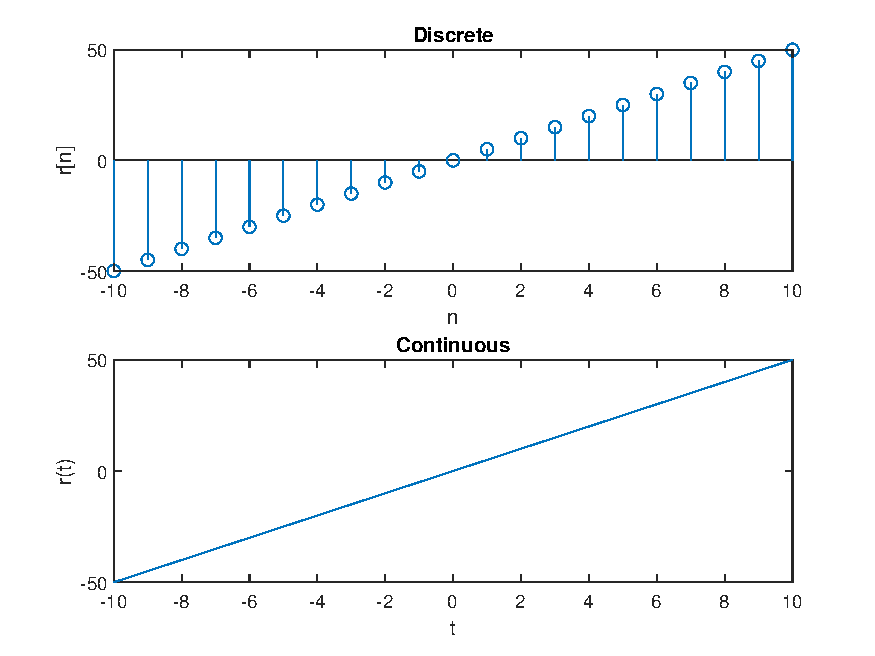
\includegraphics[scale=1.4,cframe=blue 0.5pt 3pt]{./FIG/ramp}
    \caption{Discrete and Continuous ramp Signal when a=2}
\end{figure}

% %%%%%%%%%%%%%%%%%%%%%%%%
% %%%%%%%%%%%%%%%%%%%%%%%
\subsection{Exponential Signal}
Continous time exponential signal $y(t)=ce^(at)$ and discrete time exponential signal $y[n]=ce^(an)$ were plotted using MATLAB.

\anscode{Discrete and Continuous Exponential Signal}{./CODES/exp.m}

\begin{figure}[H]
    \centering
    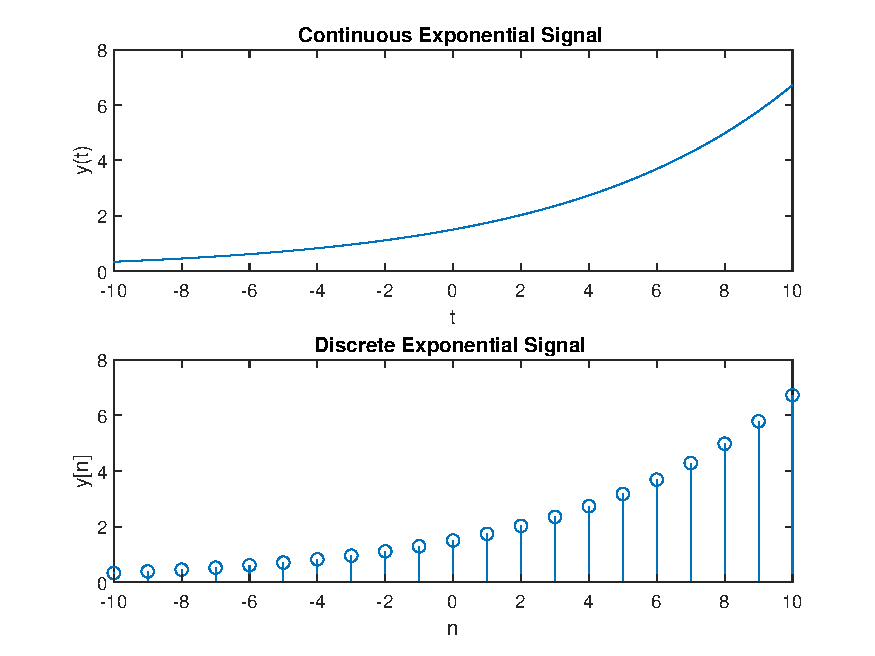
\includegraphics[scale=1.4,cframe=blue 0.5pt 3pt]{./FIG/exp}
    \caption{Discrete and Continuous Exponential Signal when c=1.5 \& a=0.15 }
\end{figure}

% %%%%%%%%%%%%%%%%%%%%%%%%
% %%%%%%%%%%%%%%%%%%%%%%%
\subsection{Unit Step Signal}
\textbf{u(t) }  \&  \textbf{ u[n] } are continuous and discrete Unit step function which has value 1 for variable(t or n) $\geqq 0$
\anscode{Discrete and Continuous Unit Step Signal}{./CODES/unit.m}

\begin{figure}[H]
    \centering
    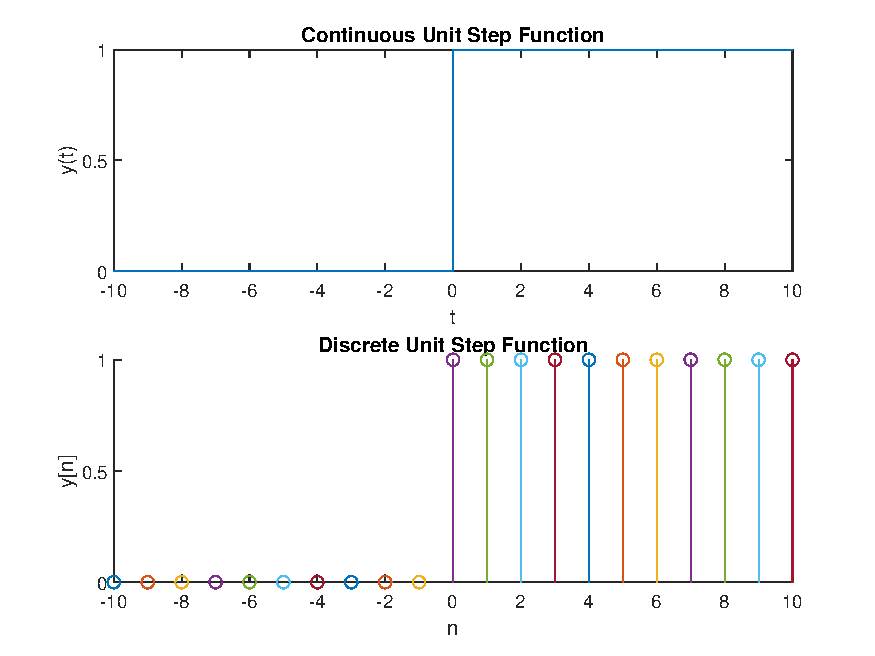
\includegraphics[scale=1.35,cframe=blue 0.5pt 3pt]{./FIG/unit}
    \caption{Discrete and Continuous Unit Step Signal}
\end{figure}

% %%%%%%%%%%%%%%%%%%%
% %%%%%%%%%%%%%%%%%%%


% %%%%%%%%%%%%%%%%%%%%%%%%%
% %%%%%%%%%%%%%%%%%%%%%%%
\section{Fourier Series}
A continuous time signal $x(t)$ with period $T$ is represented by Fourier series as

\begin{equation*}x(t)=\sum_{k = -\infty}^{\infty} a_ke^{jkw_ot}
\end{equation*}

$\quad \quad {here,w_o=2\pi/T} $\\
\begin{equation*}
    a_k=\int_{T}^{}x(t)e^{-jw_ot}  \,dx
\end{equation*}

The Fourier series representation of a square wave with period T and amplitude a is given by:
\begin{equation*}
    x(t)=\frac{4a}{\pi} \sum_{k = 1}^{\infty}\frac{sin((2k-1)w_ot)}{2k-1}
\end{equation*}

The sum of all the odd harmonics of the sinusoidal signal forms a square wave approximation.So, we varies the no of terms in summation.

\anscode{Fourier Series Representation of a Square Wave }{./CODES/FouSer.m}

\begin{figure}[H]
    \centering
    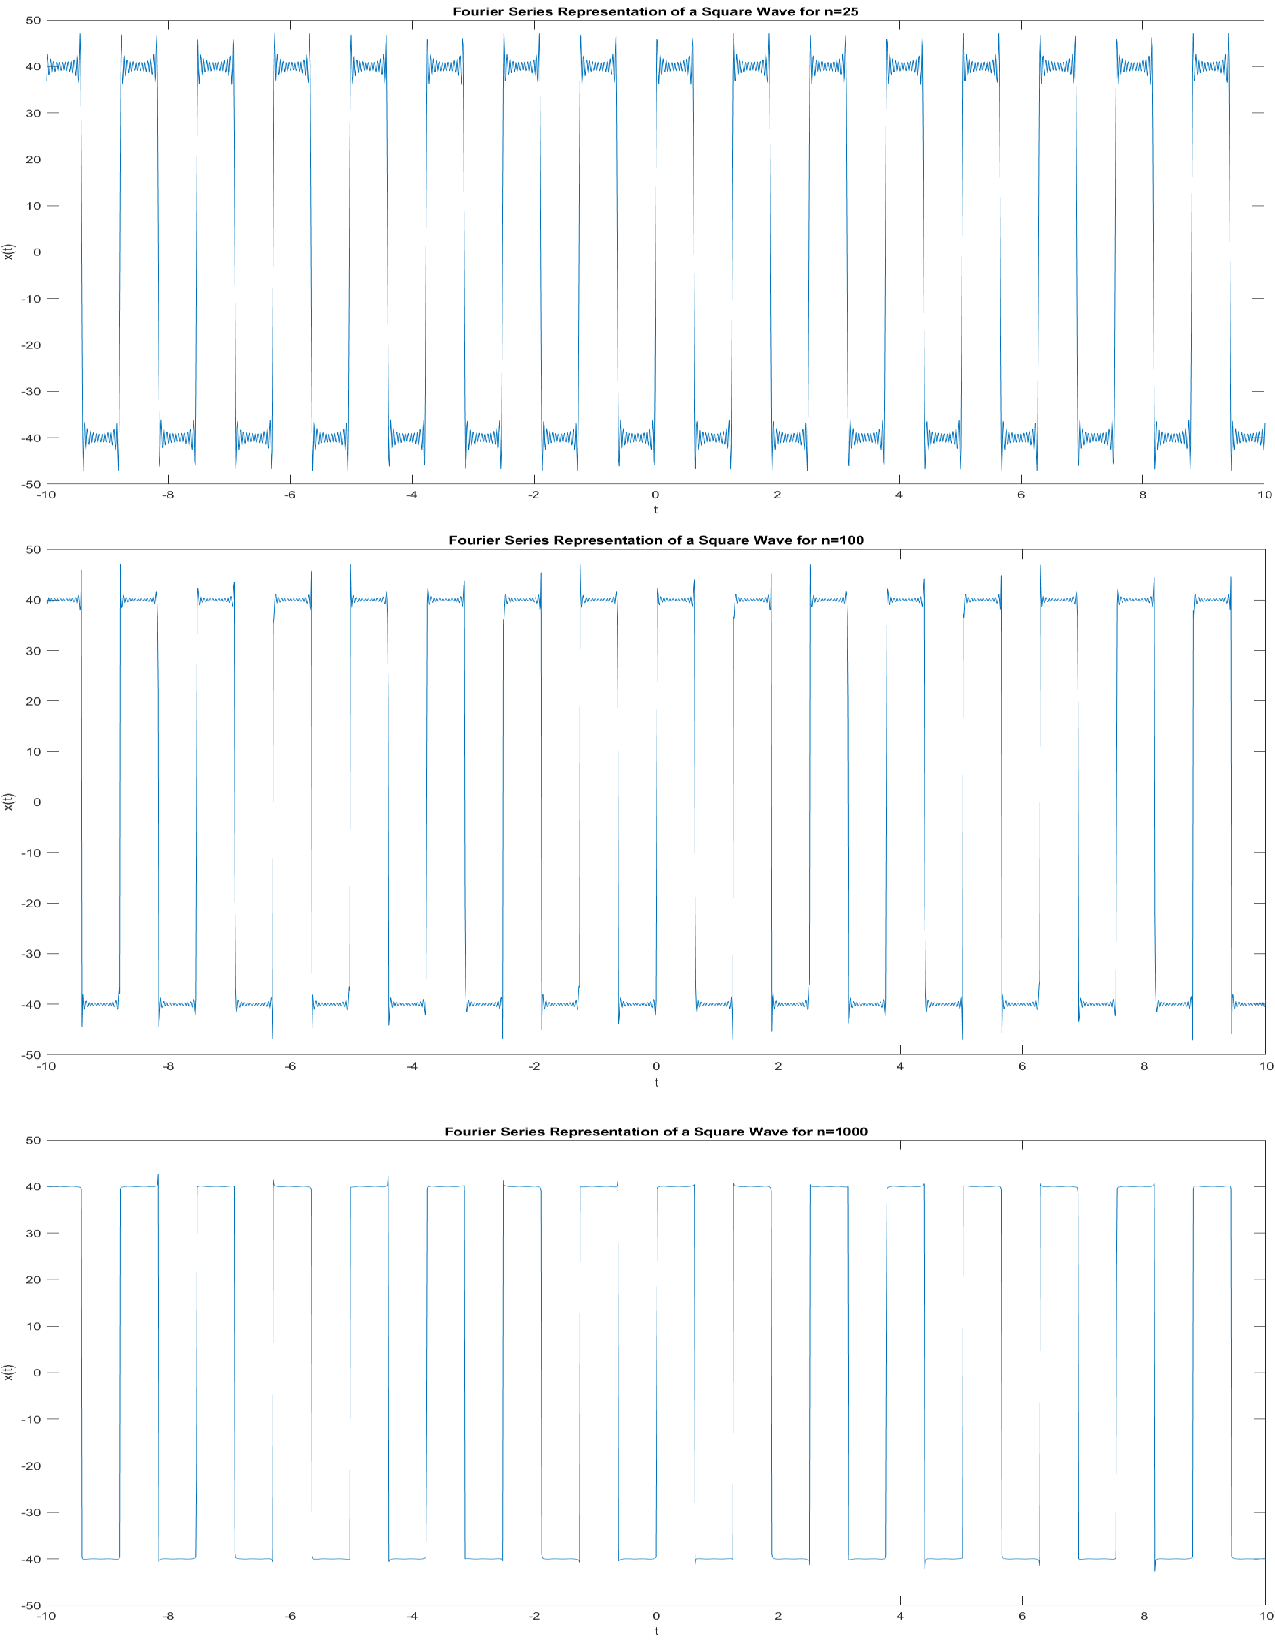
\includegraphics[scale=0.83,cframe=blue 0.5pt 3pt]{./FIG/FouSer.pdf}
    \caption{Fourier Series Representation of a Square Wave}
\end{figure}

% %%%%%%%%%%%%%%%%%%%
% %%%%%%%%%%%%%%%%%%%


% %%%%%%%%%%%%%%%%%%%%%%%%%
% %%%%%%%%%%%%%%%%%%%%%%%
\section{Fourier Transform}
The fourier transform of a continuous time signal $x(t)$ is mathematically given as,
$$
    X(j\omega) = \int_{-\infty}^{\infty} x(t) e^{-j\omega t} dt
$$
Likewise, the fourier transform of a discrete time signal $x[n]$ is mathematically given as,
$$
    X(e^{j\omega})=\sum_{n=-\infty}^{\infty} x[n] e^{-j\omega n}
$$
The \textbf{fft} function in MATLAB returns the real and imaginary parts of the fast fourier transform for the input argument. The real and imaginary parts are plotted separately.
\anscode{Fourier transform of x[n] = [0,1,2,3] }{./CODES/FouTra.m}

\begin{figure}[H]
    \centering
    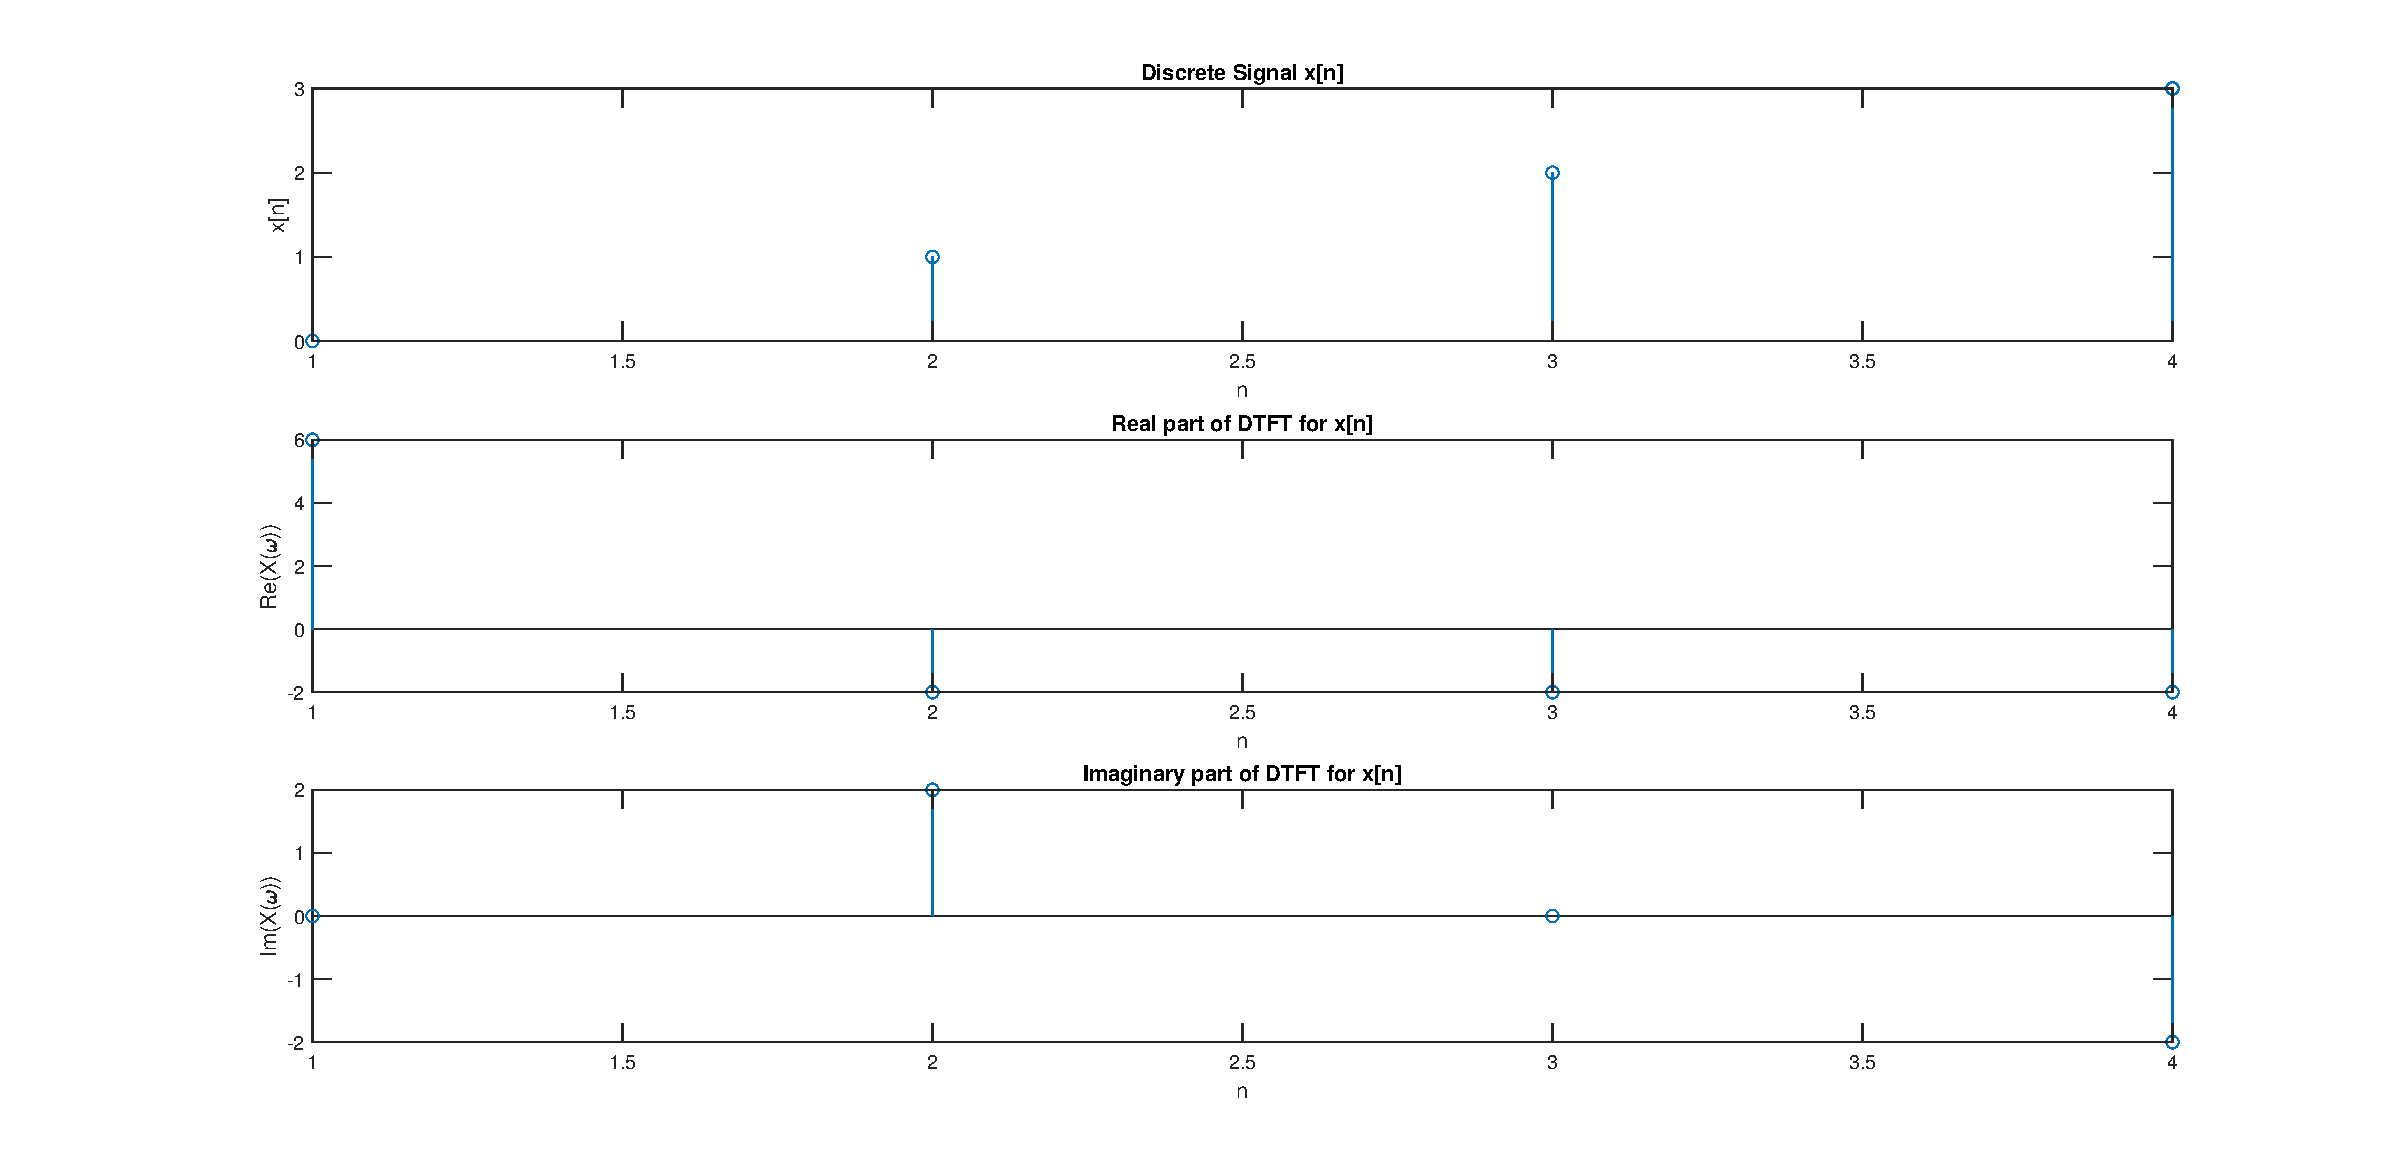
\includegraphics[scale=0.55,cframe=blue 0.5pt 3pt]{./FIG/FouTra}
    \caption{Fourier transform of x[n] = [0,1,2,3]}
\end{figure}

% %%%%%%%%%%%%%%%%%%%
% %%%%%%%%%%%%%%%%%%%

% %%%%%%%%%%%%%%%%%%%%%%%%%
% %%%%%%%%%%%%%%%%%%%%%%%
\section{Convolution}
The convolution of two continuous time signals $x(t)$ and $h(t)$, called the convolution integral, is mathematically given as,
$$
    y(t)=x(t)*h(t)=\int_{-\infty}^{\infty}x(u)h(t-u)du
$$
Likewise, the convolution of two discrete time signals $x[n]$ and $h[n]$, called the convolution sum, is mathematically given as,

$$
    y[n]=x[n]*h[n]=\sum_{k=-\infty}^{\infty} x[n]h[n-k]
$$
The \textbf{conv} function returns the convolution for two discrete sequences in MATLAB.

\anscode{Convolution for two discrete sequences $x[n]$ = [1,3,2,1,1] and $h[n]$ = [1,2,−1,1] }{./CODES/Conv1.m}

\begin{figure}[H]
    \centering
    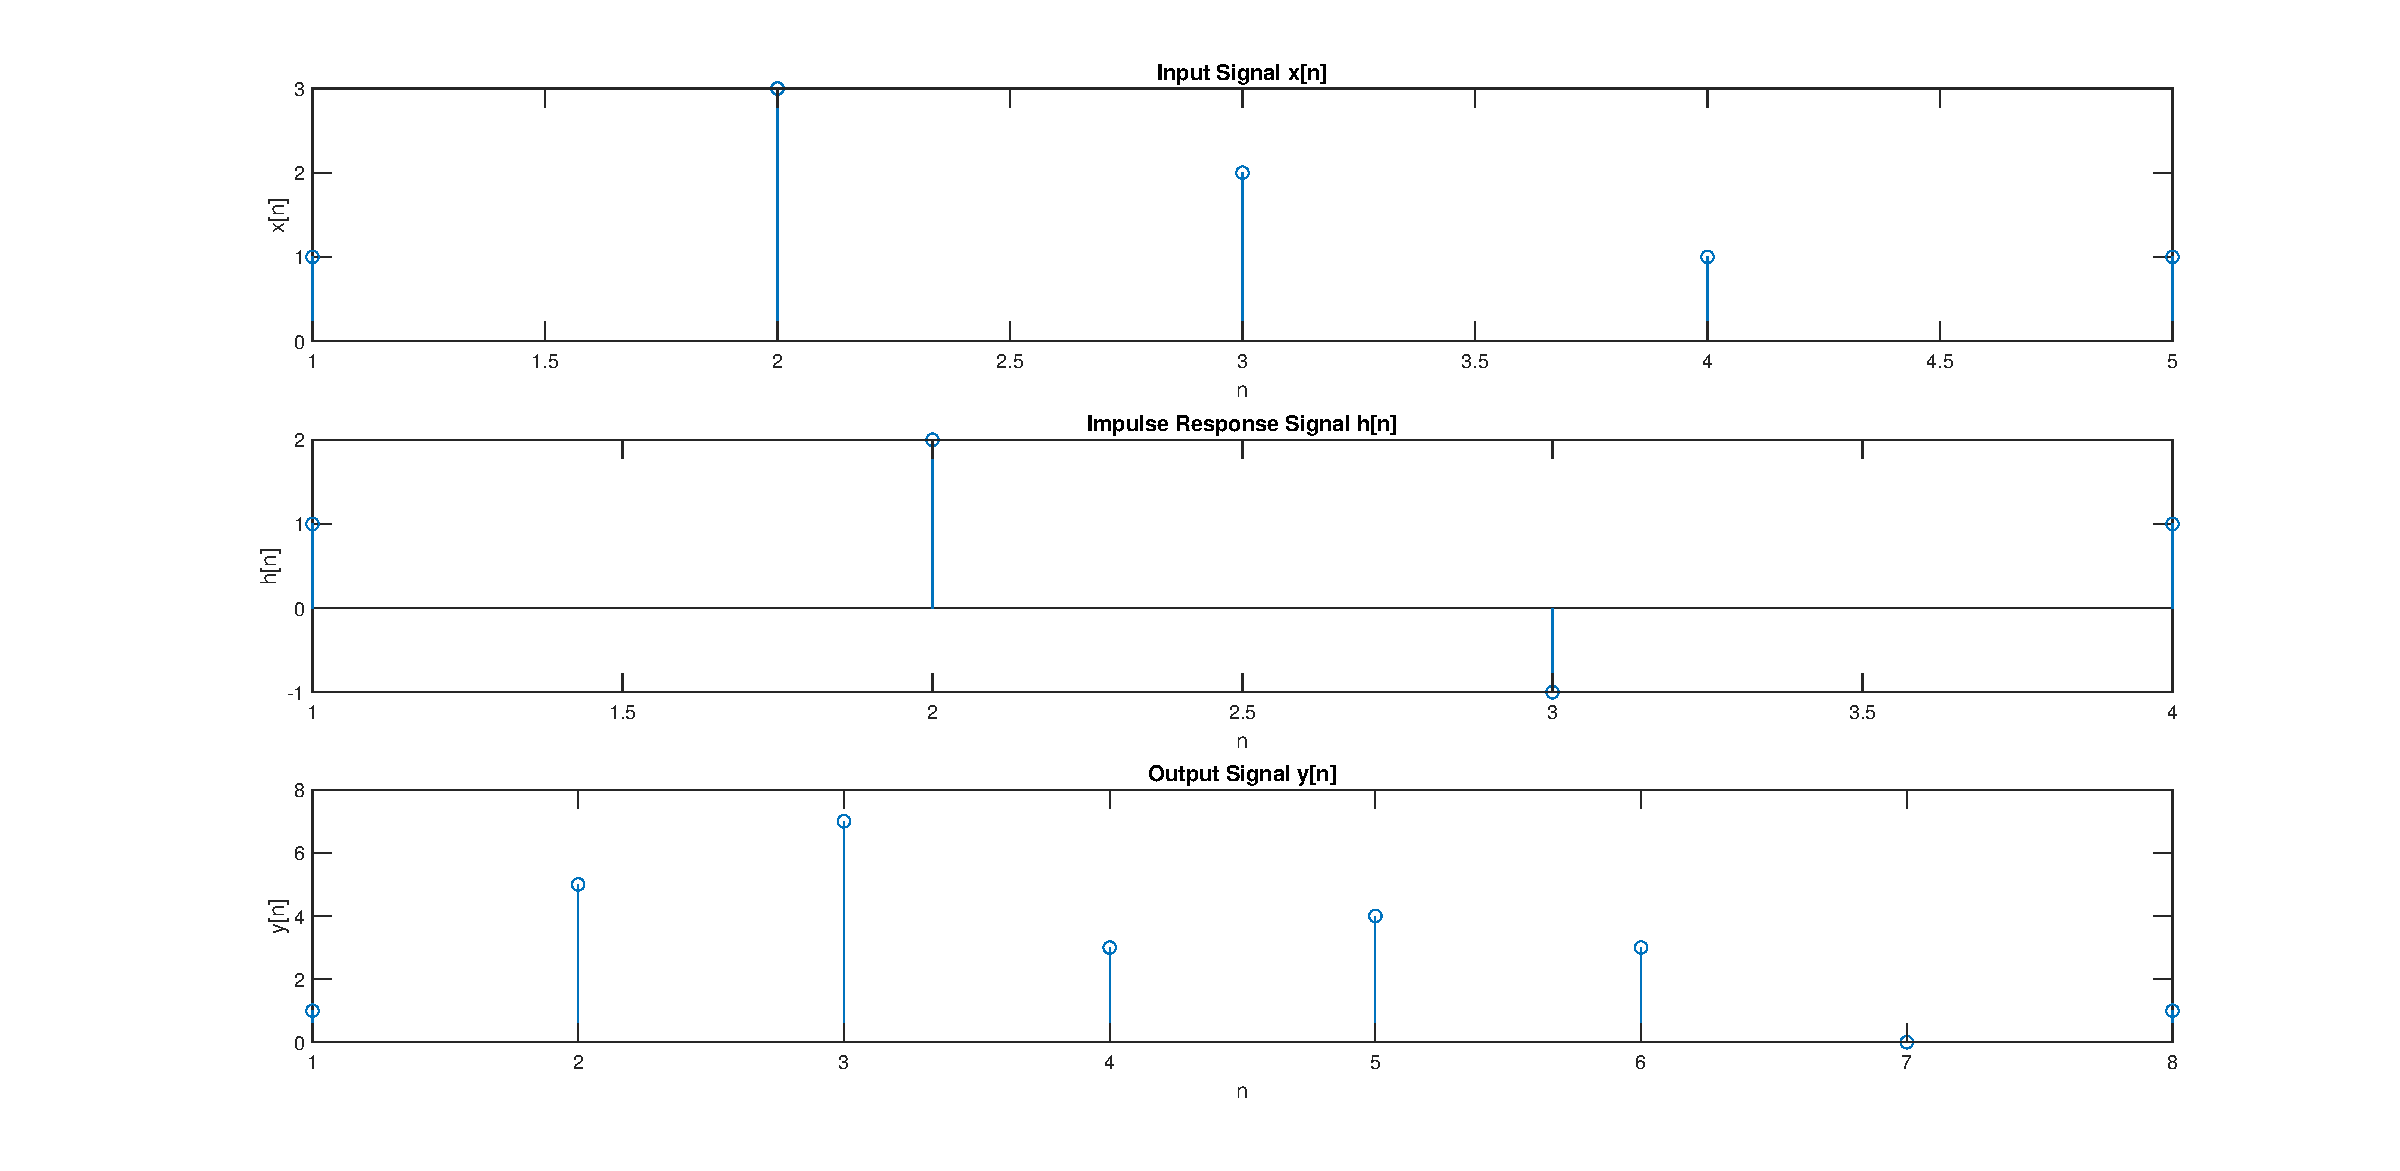
\includegraphics[scale=0.55,cframe=blue 0.5pt 3pt]{./FIG/conv1}

    \caption{Convolution for two discrete sequences $x[n]$ = [1,3,2,1,1] and $h[n]$ = [1,2,−1,1]}
\end{figure}

Convolution for two discrete sequences $x[n]$ = 0.5 n and $h[n] = u[n]$

\anscode{Convolution for two discrete sequences $x[n]$ = 0.5 n and $h[n] = u[n]$ }{./CODES/Conv2.m}

\begin{figure}[H]
    \centering
    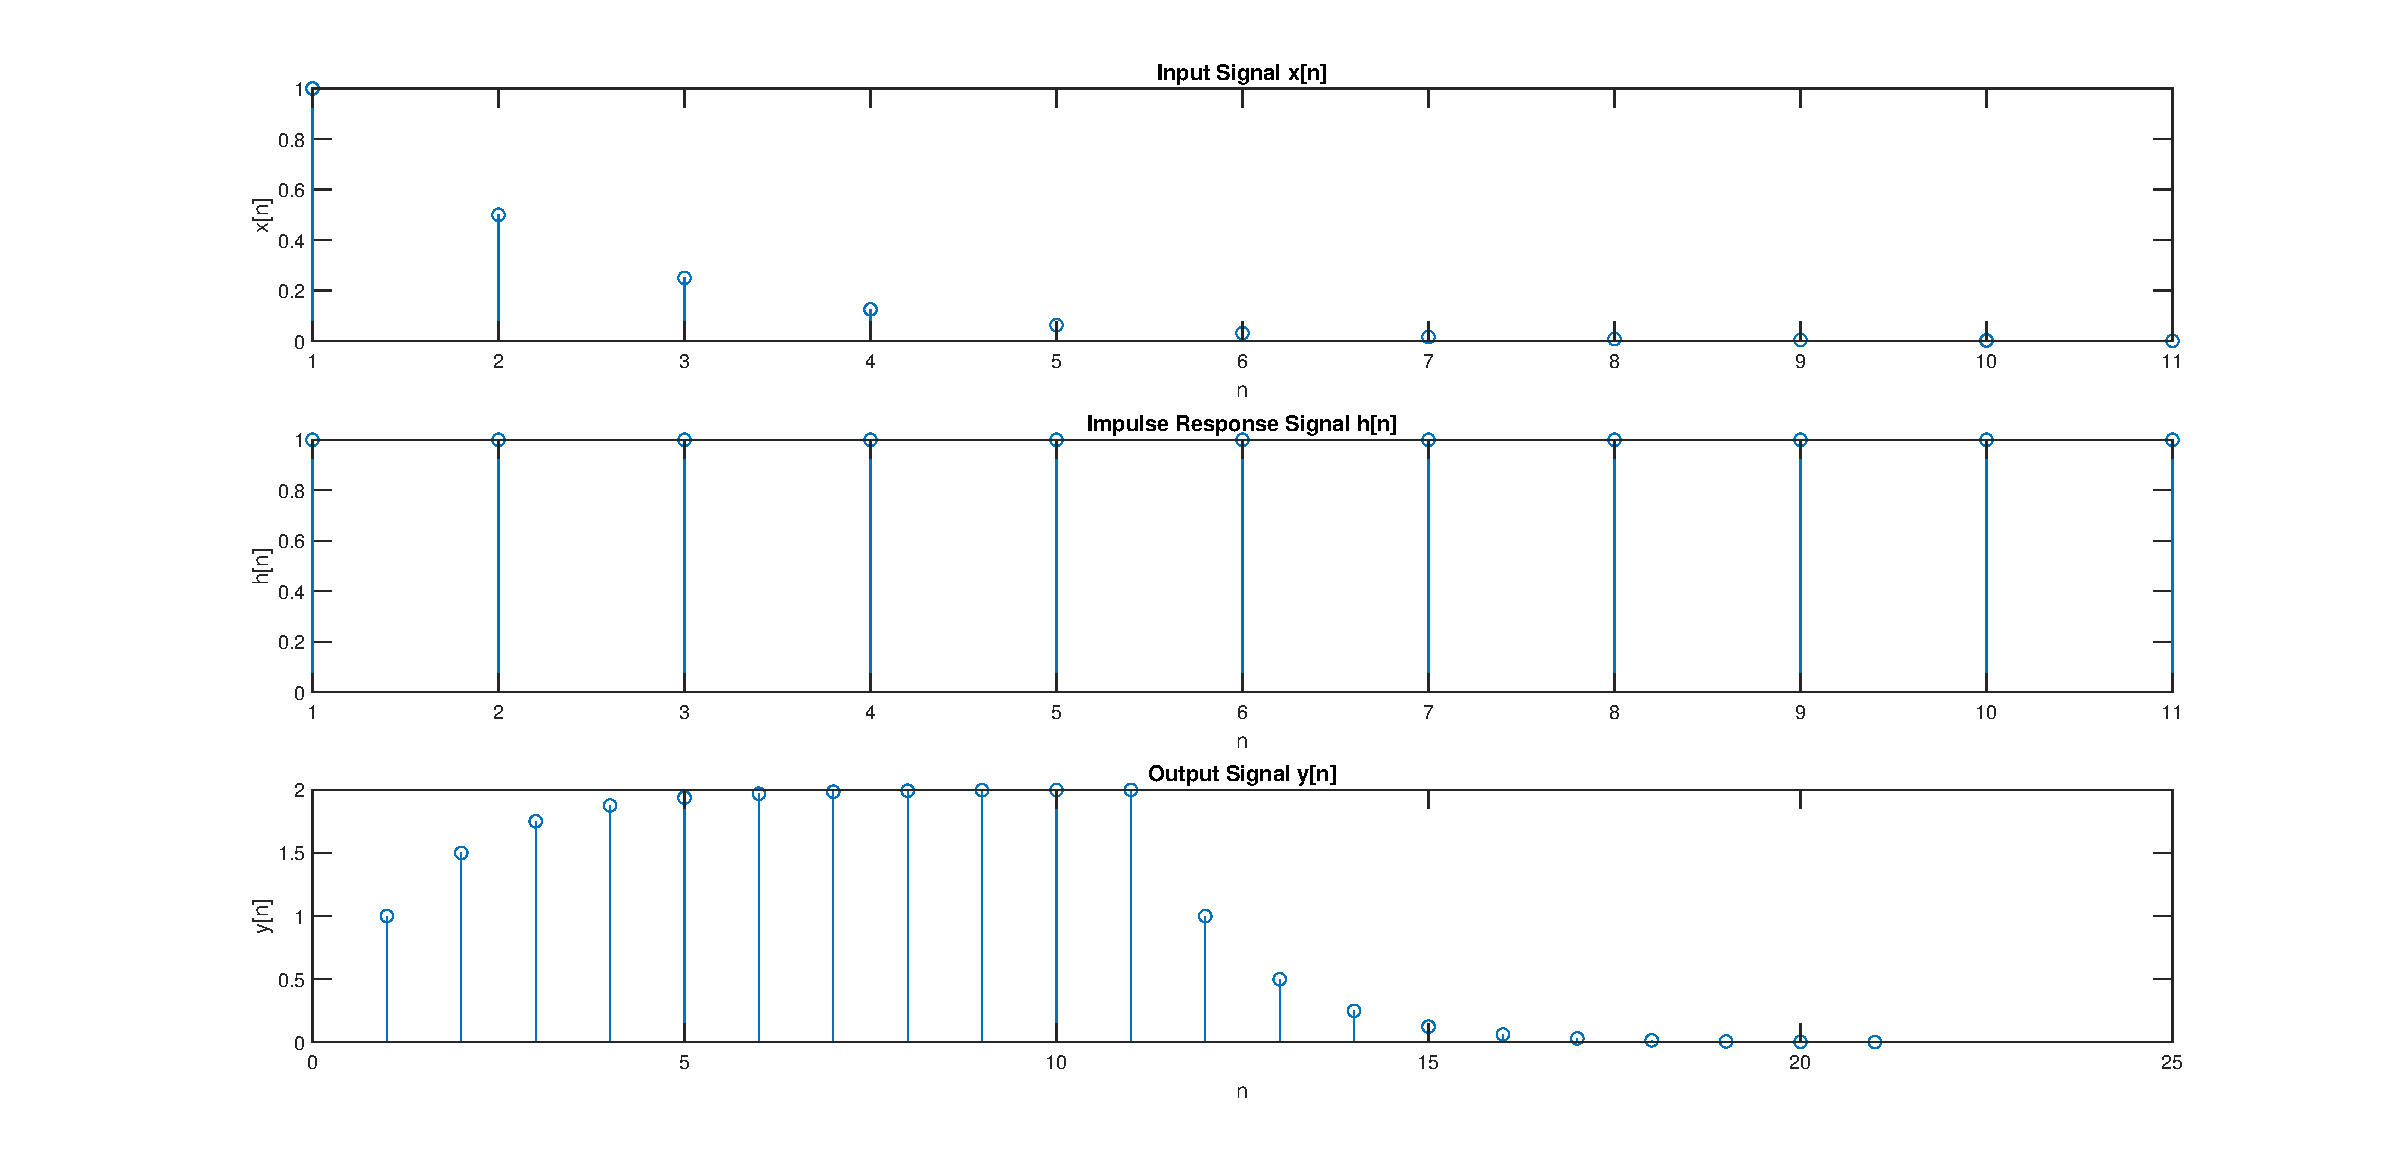
\includegraphics[scale=0.55,cframe=blue 0.5pt 3pt]{./FIG/Conv2}
    \caption{Convolution for two discrete sequences $x[n]$ = 0.5 n and $h[n] = u[n]$ }
\end{figure}

% %%%%%%%%%%%%%%%%%%%
% %%%%%%%%%%%%%%%%%%%

% %%%%%%%%%%%%%%%%%%%%%%%%%
% %%%%%%%%%%%%%%%%%%%%%%%
\section{Frequency Response of a System}
For a system with $h(t)$ as the impulse response, and $x(t)$ as the input signal, the output $y(t)$ is related to the input as the convolution,
$$
    y(t)=x(t)*h(t)=\int_{-\infty}^{\infty}x(u)h(t-u)du
$$
According to the convolution property of fourier transforms, the fourier transforms of the signals are related as,
$$
    Y(j\omega)=H(j\omega)X(j\omega)
$$
where $H(j\omega)$, the fourier transform of the impulse response of the system is the frequency response of the system. Likewise, for discrete time input signal $x[n]$ to a system with the impulse response $h[n]$, the output in frequency domain is mathematically given as,
$$
    Y(e^{j\omega})=H(e^{j\omega})X(e^{j\omega})
$$
where $H(e^{j\omega})$, the fourier transform of the impulse response of the system is the frequency response of the system.
During the lab experiment, we plotted the frequency response given as,
$$
    H(z)=\frac{0.008-0.033z+0.05z^2-0.033z^3+0.008z^4}{1+2.37z+2.7z^2+1.6z^3+0.5z^4}
$$
The \textbf{freqz} function returns the frequency response of a system whose amplitude and phase were plotted separately in MATLAB.

\anscode{ Frequency response of $H(z)$ }{./CODES/FreqRes.m}


\begin{figure}[H]

    \centering
    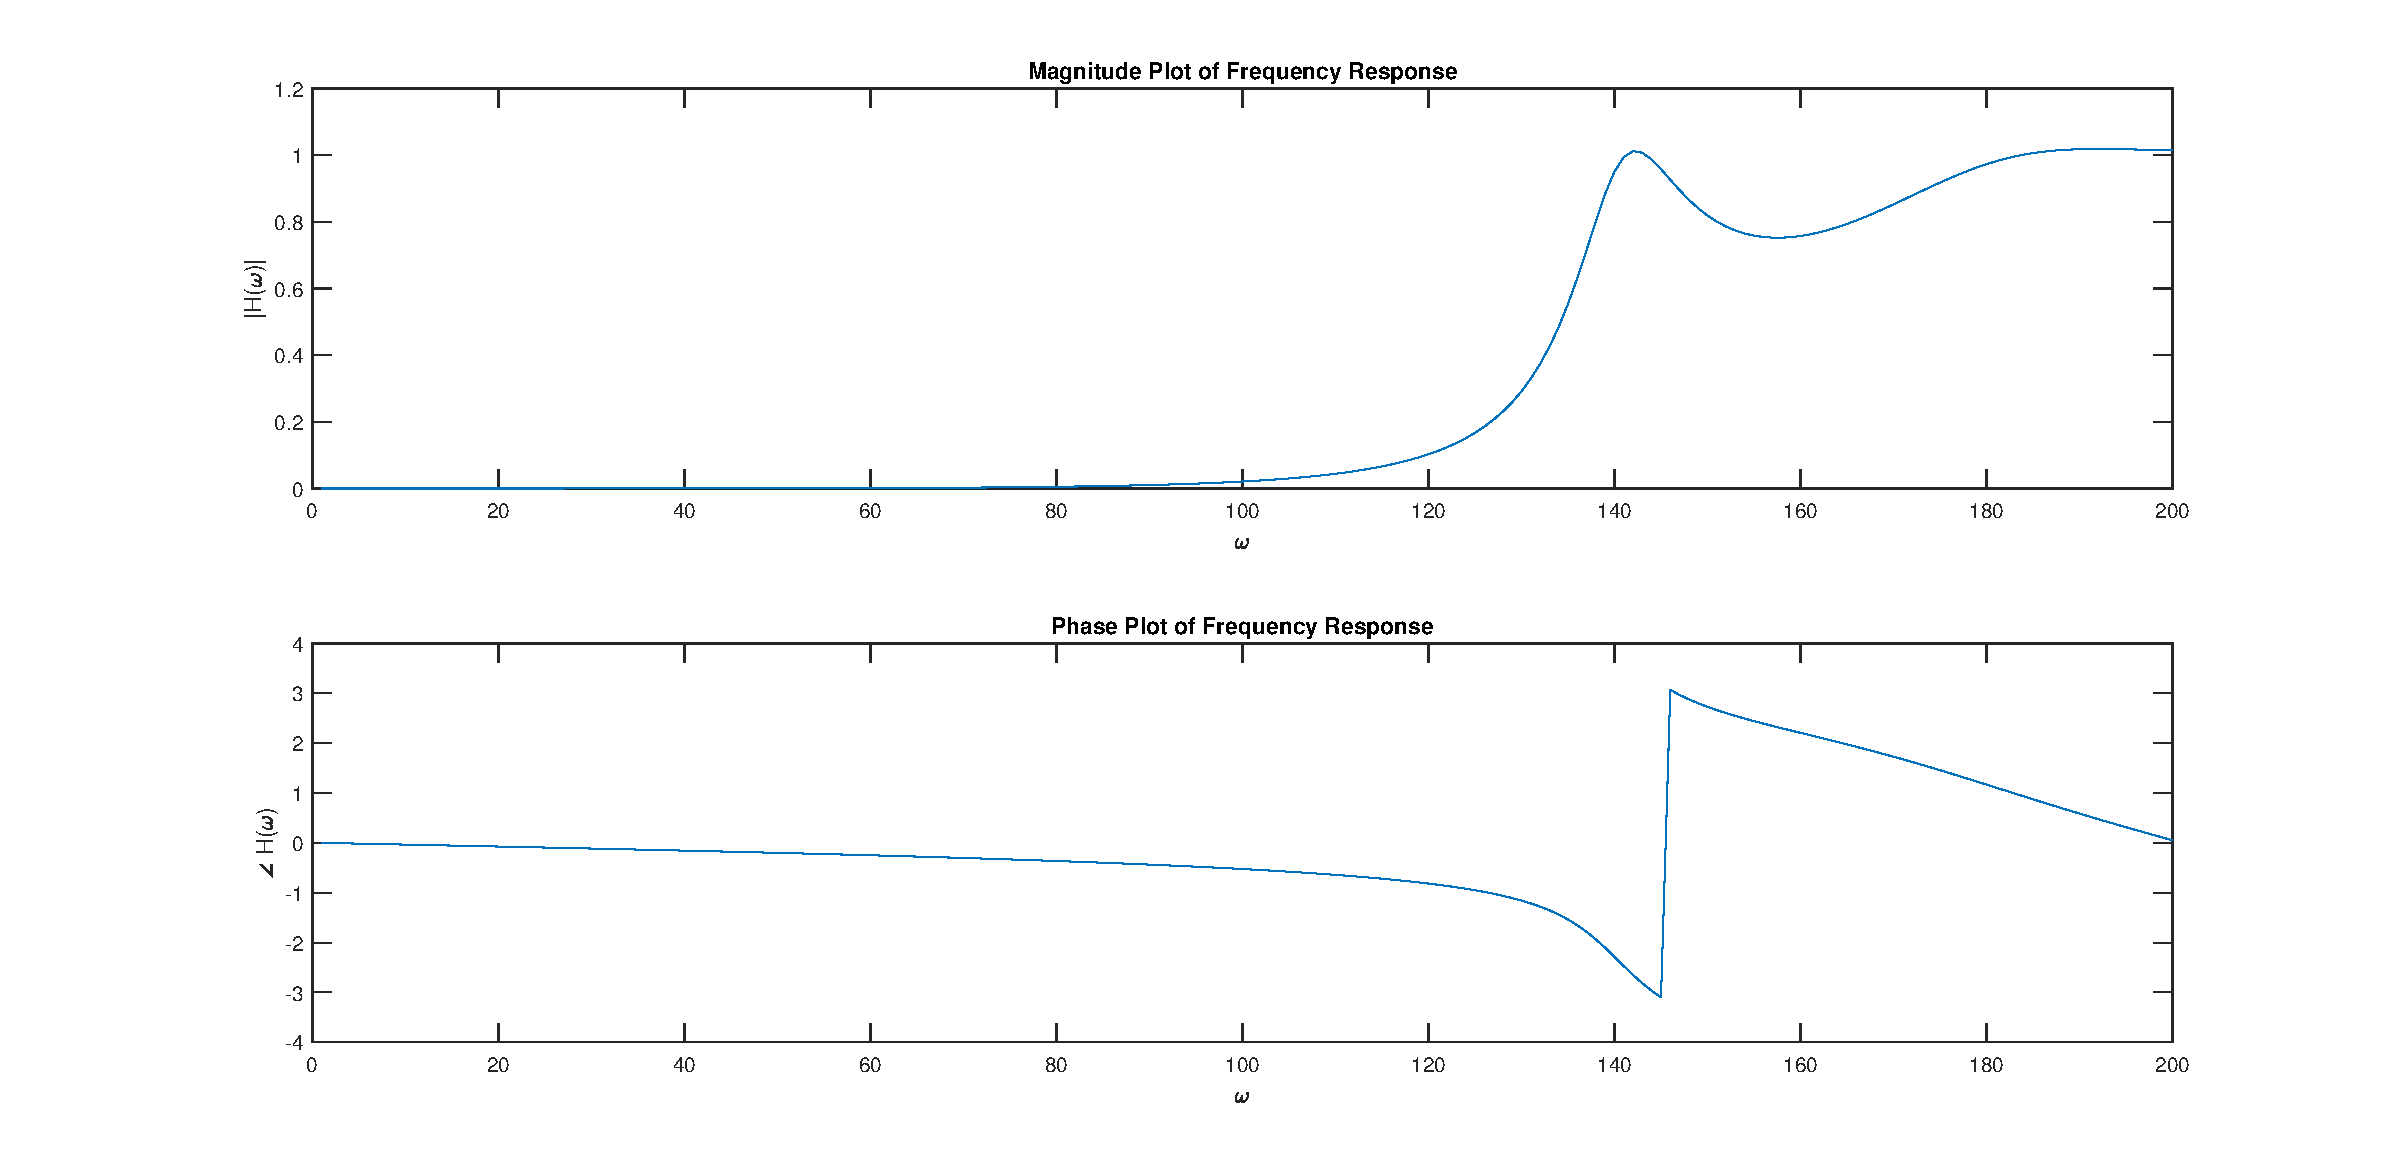
\includegraphics[scale=0.55,cframe=blue 0.5pt 3pt]{./FIG/FreqRes}
    \caption{ Frequency response of $H(z)$ }
\end{figure}

% %%%%%%%%%%%%%%%%%%%
% %%%%%%%%%%%%%%%%%%%


\section{Conclusion}
In this Lab we got familiarize to various MATLAB function. We were able to Plot some basic function like unit, exponential, Sinusoidal, Ramp etc. We also find and plot Fourier Series and Transform and additionally performed Convolution with \textbf{conv} function and view frequency response of the system. Thus all the LAB exercises were completed.


\end{document}





